\documentclass{beamer}

\mode<presentation>
{
  \usetheme{Montpellier}
  % oder ...

  \setbeamercovered{transparent}
  % oder auch nicht
}

\usepackage{array}
\usepackage[normalem]{ulem}
\usepackage{fancyvrb,verbatim}
\setlength{\extrarowheight}{2mm}

\newcommand{\vect}[2]{\ensuremath{\inp{\hspace{-.8ex}\begin{array}{c}#1\\#2\end{array}\hspace{-.4ex}}}}
\newcommand{\inp}[1]{\ensuremath{\left(#1\right)}}

%\usepackage[german]{babel}
%%\usepackage{ngerman}
% oder was auch immer

\usepackage[utf8]{inputenc}
% oder was auch immer

\usepackage{multicol}

\usepackage{times}
\usepackage[T1]{fontenc}
% Oder was auch immer. Zu beachten ist, das Font und Encoding passen
% müssen. Falls T1 nicht funktioniert, kann man versuchen, die Zeile
% mit fontenc zu löschen.

\usepackage{calc}

\title{Achieving Spin Polarization with non-magnetic Materials in Mesoscopic
Systems}

%\subtitle
%{Untertitel nur angeben, wenn es einen im Tagungsband gibt}

\author{Moritz Lenz}
\institute{Institut für Theoretische Physik und Astrophysik, Universität
Würzburg}
\date{Max Planck Institut, 2010-02-foo}

\subject{Physics}


% Falls eine Logodatei namens "university-logo-filename.xxx" vorhanden
% ist, wobei xxx ein von latex bzw. pdflatex lesbares Graphikformat
% ist, so kann man wie folgt ein Logo einfügen:

% \pgfdeclareimage[height=2.0cm]{university-logo}{Heriot-Watt_University}
% \logo{\pgfuseimage{university-logo}}



% Folgendes sollte gelöscht werden, wenn man nicht am Anfang jedes
% Unterabschnitts die Gliederung nochmal sehen möchte.
%\AtBeginSubsection[]
%{
%  \begin{frame}<beamer>
%    \frametitle{Gliederung}
%    \tableofcontents[currentsection,currentsubsection]
%  \end{frame}
%}


% Falls Aufzählungen immer schrittweise gezeigt werden sollen, kann
% folgendes Kommando benutzt werden:

%\beamerdefaultoverlayspecification{<+->}



\begin{document}

\begin{frame}
  \titlepage

  \begin{center}
{ 	
	 Diploma Thesis\\[1.5em]
}
    Supervisor: Prof. Ewelina Hankiewicz

\end{center}

%  \begin{multicols}{2}
%  \includegraphics[width=0.4\textwidth]{setup-79_reduced.jpg}
%
%{  \tiny Graphics from 
%	http://www.quantumlah.org/images/
%	setup-79\_800x600.jpg}
%  \end{multicols}

\end{frame}

\section{Motivation}

\begin{frame}
    \frametitle{Motivation - Why spin manipulation}

	\begin{itemize}
		\item Spin states can encode information
		\item Spin states stay coherent much longer than charge states
        \item Now moving required to change state
        \item Less heat dissipation
	\end{itemize}

\end{frame}

\subsection{Ferromagentic materials}

\begin{frame}{Motivation - Achievements of Spintronics}
        \textbf{Giant Magnetoresistance}

    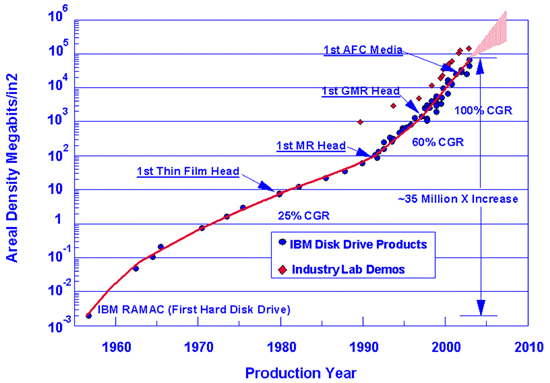
\includegraphics[width=75mm]{storage-density.png}

    \footnotesize DOI: 10.1081/E-ENN-120006100
\end{frame}

% TODO frame with Datta-Das transistor
\begin{frame}{Motivation - Achievements of Spintronics}
    \textbf{Datta-Das Transistor}

    TODO

\end{frame}

\begin{frame}{Motivation - Prior Art}
    \textbf{Why investigate alternatives?}

	\begin{itemize}
		\item Technologically hard to handle
        \item Limits in scaling down
        \item Static effects only
		\item Ferromagnetic materials are metals
            $\Rightarrow$ Schottky junctions when mixing with semiconductors
	\end{itemize}
\end{frame}

\subsection{Non-magnetic semiconductors}
\begin{frame}{Motivation - Alternatives}
    \textbf{Spin manipulation in non-magnetic semiconductors}

	\begin{itemize}
		\item Well-known techniques applicable
        \item Asymmetry tunable by electric fields
        \item Analogy to optics
	\end{itemize}
\end{frame}

\section{Theory}
\subsection{Relativistic quantum theory}
\begin{frame}{Theory: Pauli Equation}
    Relativistic QM in vacuum

    \begin{align*}
        \left( \frac{\vec p^2}{2m}- \frac{e\hbar \ \vec\sigma \cdot (\vec p \times \vec E)}
                        {2\Delta} +\ldots\right)\Psi = E \Psi
    \end{align*}

    \begin{align*}
        \Delta\qquad       & 2m_e c^2\\
        \vec \sigma \qquad & \textnormal{Pauli matrices}\\
        \vec p      \qquad & \textnormal{momentum}\\
        \vec E      \qquad & \textnormal{electric field}\\
    \end{align*}

\end{frame}

\subsection{Rasbha spin-orbit coupling}

\begin{frame}{Theory:  Bychkov-Rashba term}
    In Solids

    \begin{align*}
        H = \frac{\vec p^2}{2 m^*} + \alpha (\vec I \times \vec \sigma) \cdot
        \vec p
    \end{align*}

    \begin{align*}
        \alpha  \qquad & \textnormal{SO-coupling strength}\\
        \vec I  \qquad & \textnormal{Unit vector of asymmetry}
    \end{align*}

\end{frame}

\begin{frame}{Theory: Dispersion relation and Rashba}

    \begin{multicols}{2}
        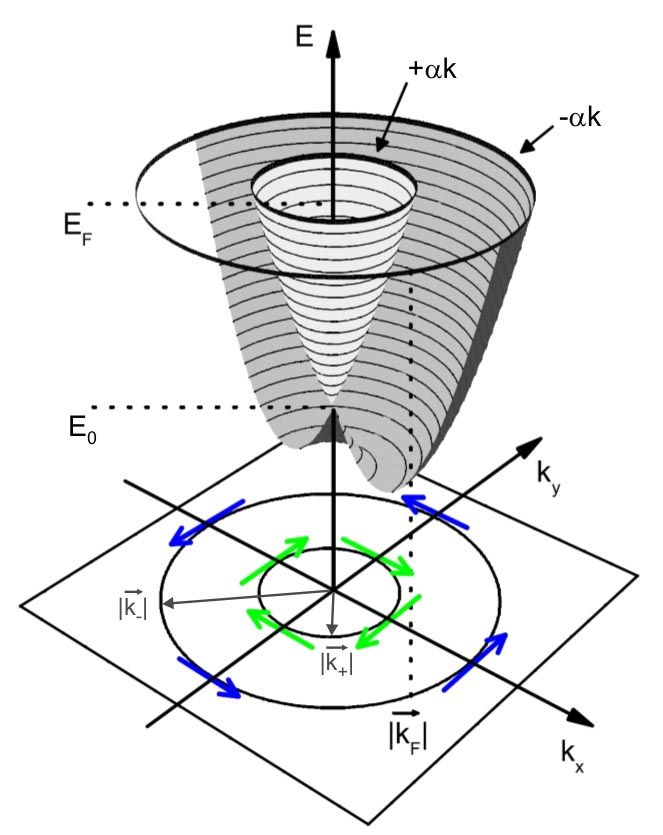
\includegraphics[height=6cm]{rashba-dispersion.jpg}

        \begin{align*}
            E(k) = \frac{\hbar^2}{2 m^*} k^2 \pm \alpha k
        \end{align*}

        Energy depends on spin and momentum $\Rightarrow$ manipulable\\[1em]

        $\alpha$ tunable through external electric field.
\end{multicols}
\end{frame}

\subsection{Landauer Formula}

\begin{frame}{Theory: Landauer Formula}
    \begin{multicols}{2}
        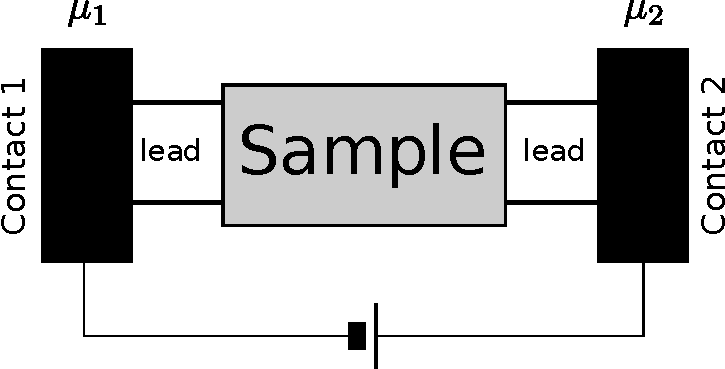
\includegraphics[width=6cm]{sample-leads}

        \begin{align*}
            G = \frac{2 e^2}{h} MT
        \end{align*}

        \begin{align*}
            G \qquad& \textnormal{conductance}\\
            M \qquad& \textnormal{number of modes}\\
            T \qquad& \textnormal{transmission propability}
        \end{align*}
    \end{multicols}
\end{frame}

\begin{frame}{Theory: Green's Function formalism}
    \begin{multicols}{2}
        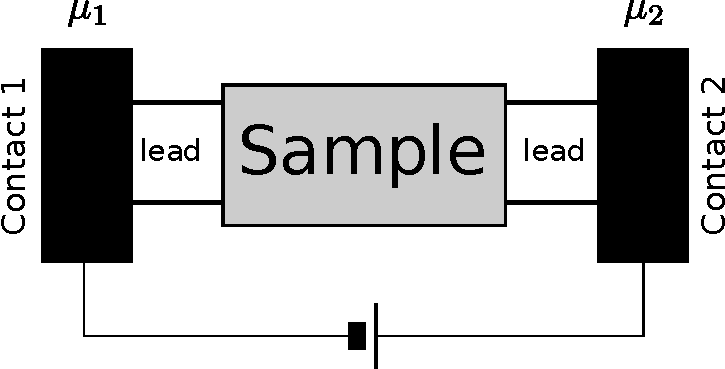
\includegraphics[width=6cm]{sample-leads}

        \begin{align*}
            G = \frac{2 e^2}{h} MT
        \end{align*}

        \begin{align*}
            G \qquad& \textnormal{conductance}\\
            M \qquad& \textnormal{number of modes}\\
            T \qquad& \textnormal{transmission propability}
        \end{align*}
    \end{multicols}
\end{frame}

\begin{frame}{Theory: Green's Functions}
    \begin{center}
        Inhomogeneous Schrödinger equation
        \begin{align*}
            (E-H) \Psi &= \delta(x-x_0)\\
            \Psi       &= \underbrace{(E-H)^{-1}}_{G} \delta(x-x_0)
        \end{align*}
        \pause
        \begin{align*}
            G^R = ((E + i \eta) -H)^{-1}\quad & \textnormal{wave moving away from exitation}\\
            G^A = ((E - i \eta) -H)^{-1}\quad & \textnormal{wave moving
            towards exitation}
        \end{align*}

        \begin{align*}
        \end{align*}
   \end{center}
\end{frame}

\begin{frame}{Theory: Coupling}
    Problem: $(E\pm i\eta-H)$ is an operator, and not easily invertible\\[1em]

    \pause
    Solution: discretize derivative into finite differences\\[1em]

    \pause
    Leads: Analytical Green's functions known\\[1em]

    \pause
    Describe coupling between leads and sample by matrices $\Sigma_p$
\end{frame}

\begin{frame}{Theory: Fisher-Lee Relation}
    \huge
    \begin{align*}
        T_{pq} = \textnormal{Trace}( \Sigma_p G^R \Sigma_q G^A )
    \end{align*}
\end{frame}

\section{Work done}
\begin{frame}{Setup}
    \begin{itemize}
        \item 2D electron gas in quantum well
        \item 2 bands considered
        \item $T = 0$
        \item size: about 200nm
        \item ballistic transport
        \item coherent transport
        \item Interface between SO and normal regimes
    \end{itemize}
\end{frame}

\subsection{Analytical calculations}

\begin{frame}{Analytical calculations}
    \begin{multicols}{2}
        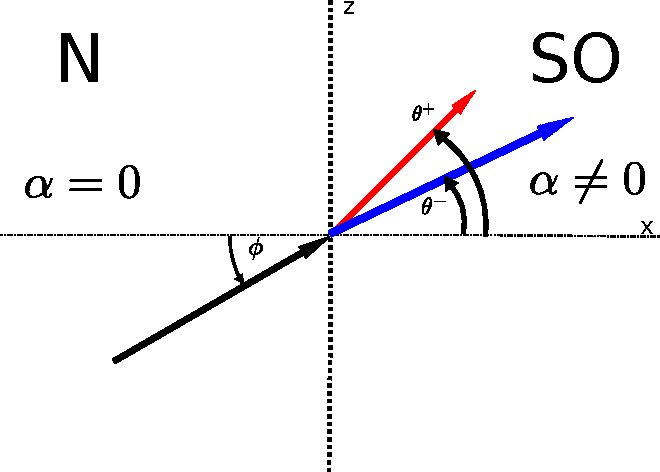
\includegraphics[width=55mm]{setup-simple}

    \begin{align*}
        H_r &= \frac{p^2}{2m} + (-\vec y \times \vec \sigma) \cdot
                \alpha(x) \vec p\\ 
        E_{\pm} &= \frac{p^2}{2m} \pm \alpha \\
        v_{\pm} &= \frac{\partial E_{\pm}}{\partial p} = \frac{p}{m} \pm \alpha
    \end{align*}

    \end{multicols}
\end{frame}


\begin{frame}{Analytical calculations - Wave functions}
    \begin{align*}
    \chi_{SO}^{\pm} &= \frac{1}{n_{SO}^{\pm}} 
                        \vect{-p_{x,SO}^{\pm} \pm p_{SO}^\pm}{p_z} \\
        n_{SO}^{\pm}   &= \sqrt{|-p_{x,SO}^{\pm} \pm p_{SO}^\pm|^2 +
            p_z^2}
    \end{align*}
    \pause
    \begin{align*}
        \Psi^+ = e^{i p_z z} * \left\{
            \begin{array}{ll}
                e^{i p_x x} \chi_N^+ + e^{- i p_x x} (\chi_N^+ r_{++} +
                        \chi_N^- r_{-+})    & x < 0\\
                e^{i p_x^+ x} \chi_{SO}^+ t_{++} + e^{i p_x^- x}
                \chi_{SO}^- t_{-+}          & x > 0
            \end{array} \right.
    \end{align*}


\end{frame}

\end{document}
